\chapter{Tests und Experimente}
\label{cha:tests}

Im Kapitel Tests und Experimente werden unterschiedliche Hyperparameter-Konfigurationen auf ihre Auswirkungen getestet. Außerdem wird mit unterschiedlichen
Netzwerk-Architekturen die Performanz auf Geräten mit leistungsarmer Hardware gemessen.

\section{Auswirkungen der Hyperparameter}

Im Folgenden werden unterschiedliche Kombinationen der Gewichtungsparameter Content-Weight $ \alpha $, Style-Weight $ \beta $ und Total-Variation-Weight $ \gamma $ getestet. Dabei wird als Inhaltsbild  eine eigene Abbildung der HTW-Berlin benutzt. Als Stilbild wird das Kunstwerk \textit{Starry Night} des Künstlers Vincent Van Gogh und \textit{The Scream} von Edvard Munch verwendet. Die generierten Bilder entsprechen einer Größe von 768 * 768 Pixeln. Die restlichen Hyperparameter werden aus dem Kapitel Methodologie \ref{sec:method_neural_style_transfer} übernommen.

\pagebreak

\subsection{Experiment 1: Starry Night}

In diesem Experiment wird das Stilbild Starry Night von Vincent Van Gogh verwendet.

\begin{figure}[H]
    \centering
    \begin{subfigure}[h]{0.20\textwidth}
        \centering
        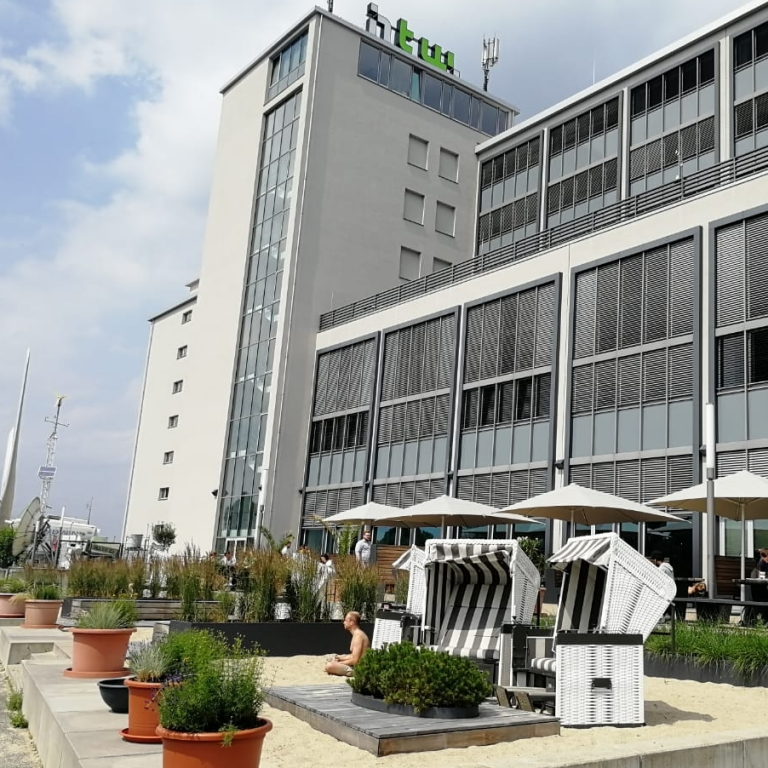
\includegraphics[width=\textwidth]{resources/content/content/htw-768x768.jpg}
    \end{subfigure}
    \begin{subfigure}[h]{0.20\textwidth}
        \centering
        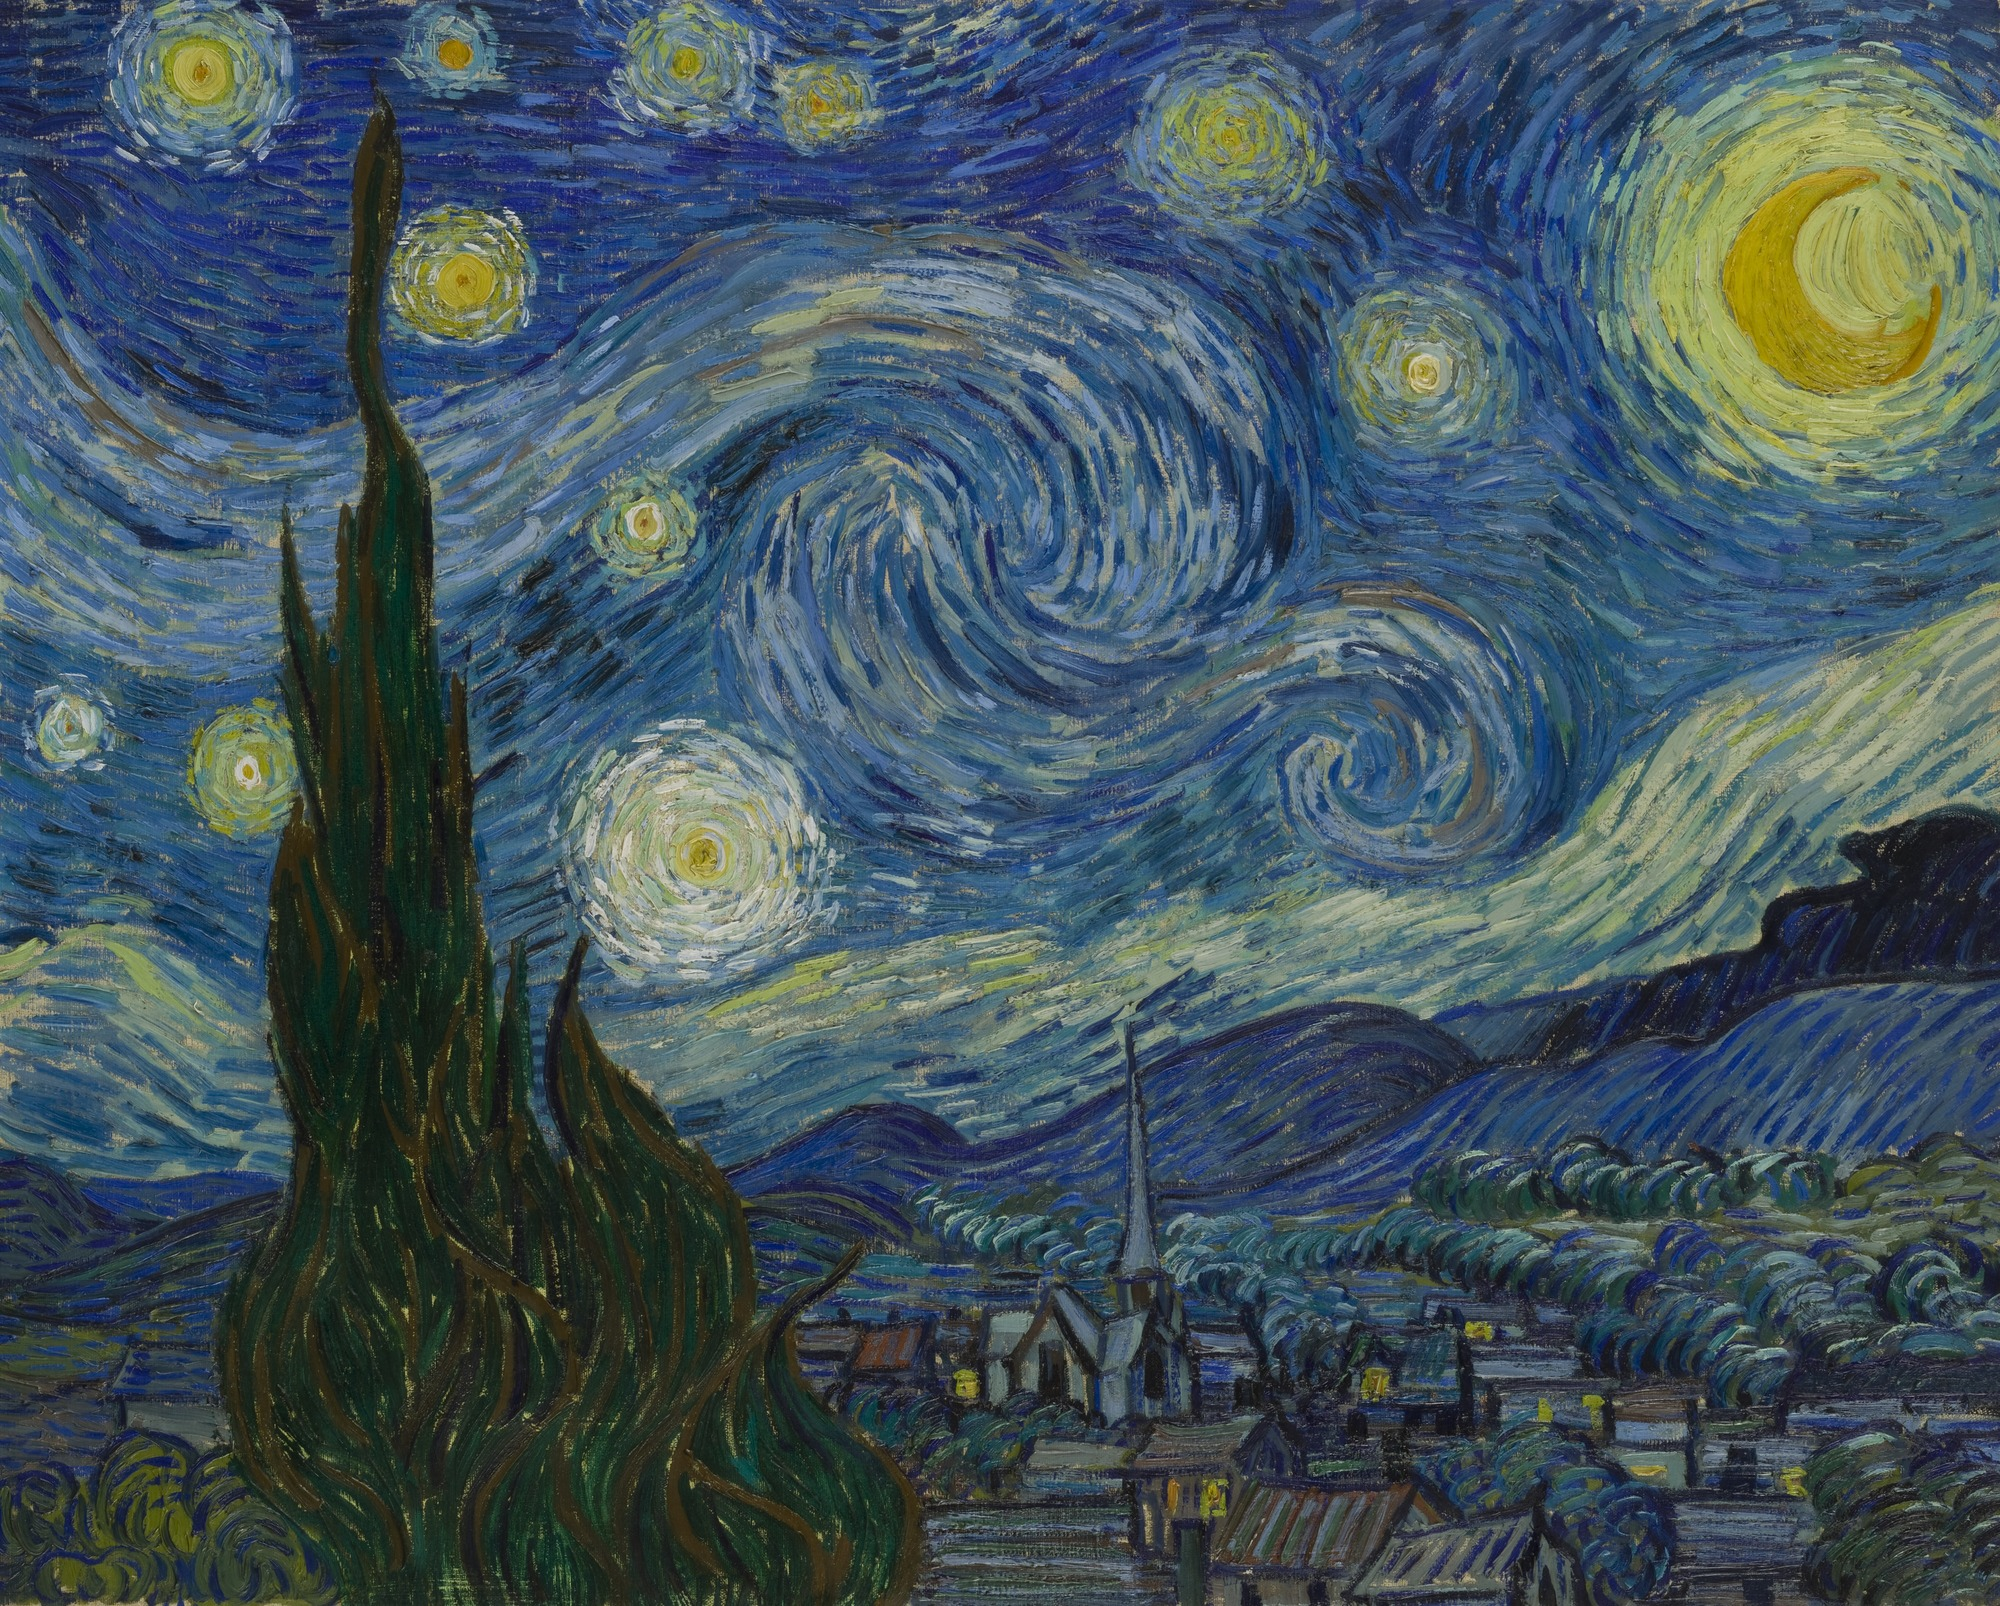
\includegraphics[width=\textwidth]{resources/content/style/starry_night.jpg}
    \end{subfigure}
    \caption{HTW kombiniert mit Starry Night}
\end{figure}

In der ersten Abbildungen werden verschiedene die verschiedenen  \\
Stilgewichtungen $ \beta = 10^{5} $, $ \beta = 10^{6} $, $ \beta = 10^{7} $, $ \beta = 10^{8} $ und $ \beta = 10^{9} $ für Starry Night getestet.

\begin{figure}[H]
    \centering
    \begin{subfigure}[h]{0.15\textwidth}
        \centering
        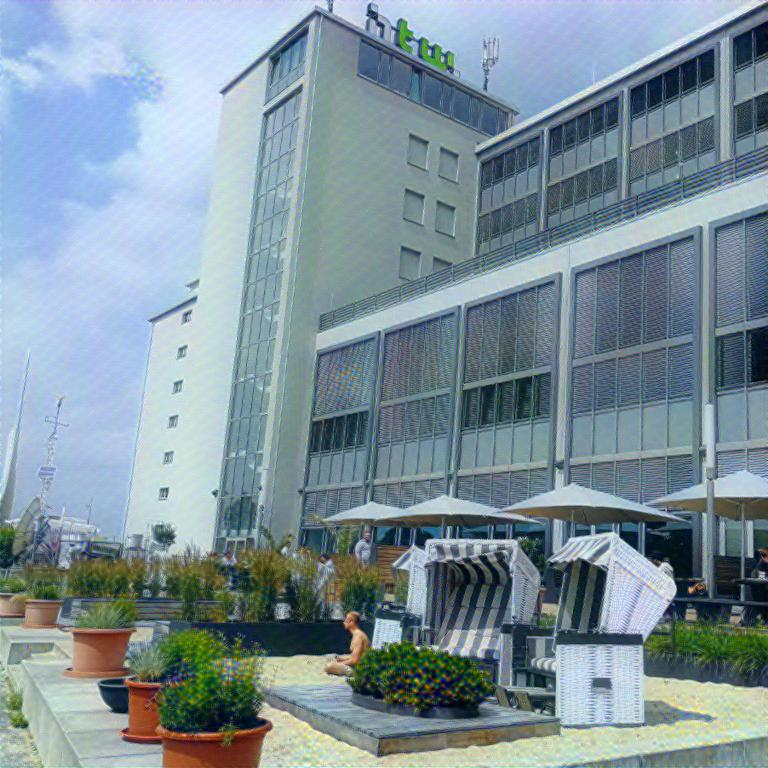
\includegraphics[width=\textwidth]{resources/content/experiments/a__starry_night__768x768__style-weight_1e+05__tv-weight_0e+00.jpg}
    \end{subfigure}
    \begin{subfigure}[h]{0.15\textwidth}
        \centering
        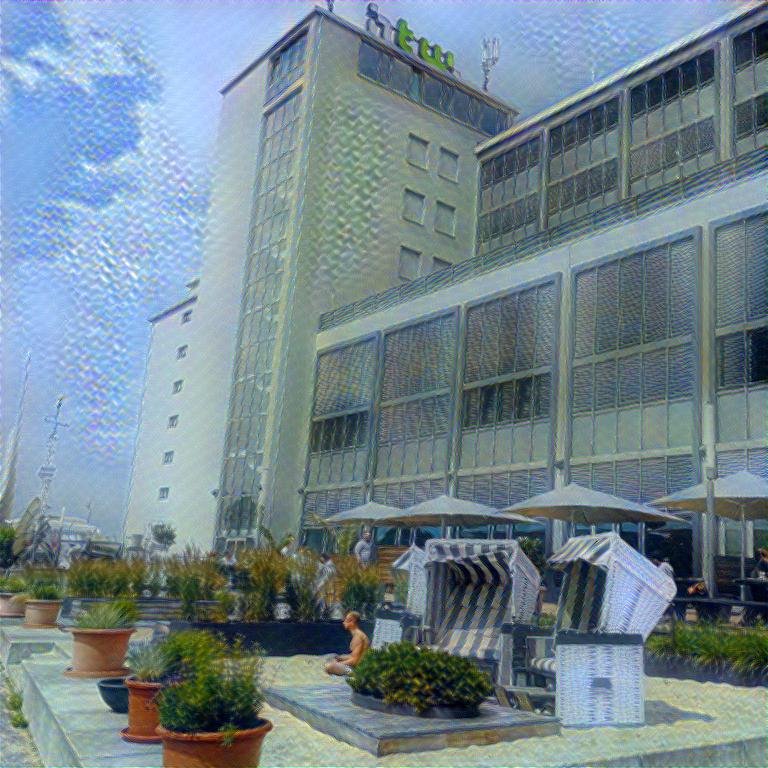
\includegraphics[width=\textwidth]{resources/content/experiments/a__starry_night__768x768__style-weight_1e+06__tv-weight_0e+00.jpg}
    \end{subfigure}
    \begin{subfigure}[h]{0.15\textwidth}
        \centering
        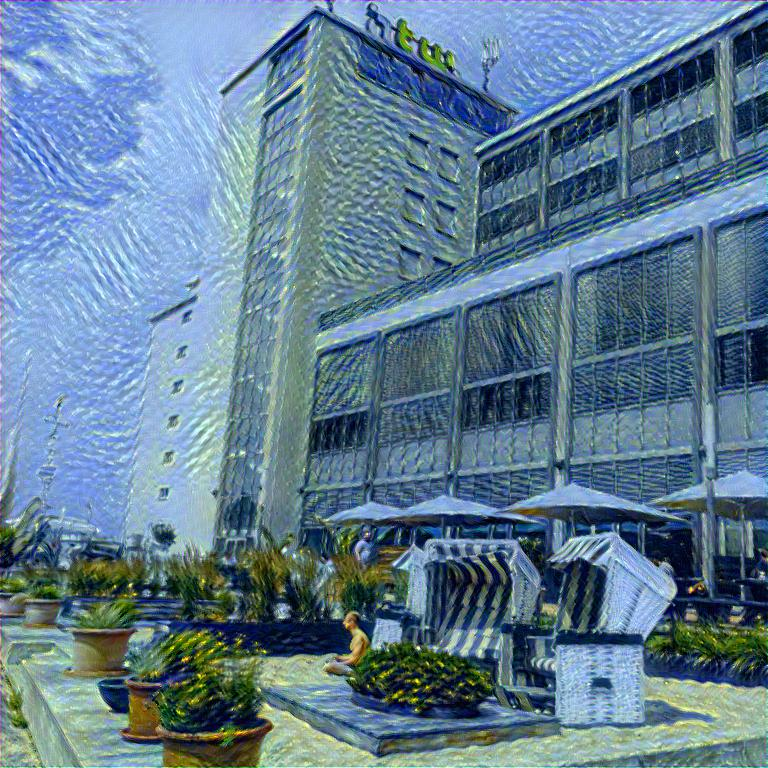
\includegraphics[width=\textwidth]{resources/content/experiments/a__starry_night__768x768__style-weight_1e+07__tv-weight_0e+00.jpg}
    \end{subfigure}
    \begin{subfigure}[h]{0.15\textwidth}
        \centering
        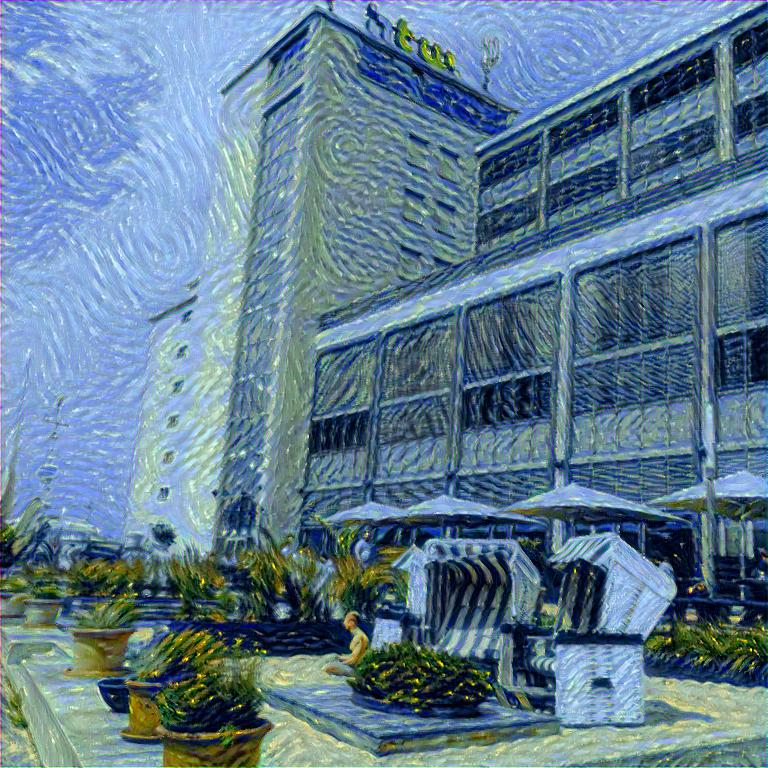
\includegraphics[width=\textwidth]{resources/content/experiments/a__starry_night__768x768__style-weight_1e+08__tv-weight_0e+00.jpg}
    \end{subfigure}
    \begin{subfigure}[h]{0.15\textwidth}
        \centering
        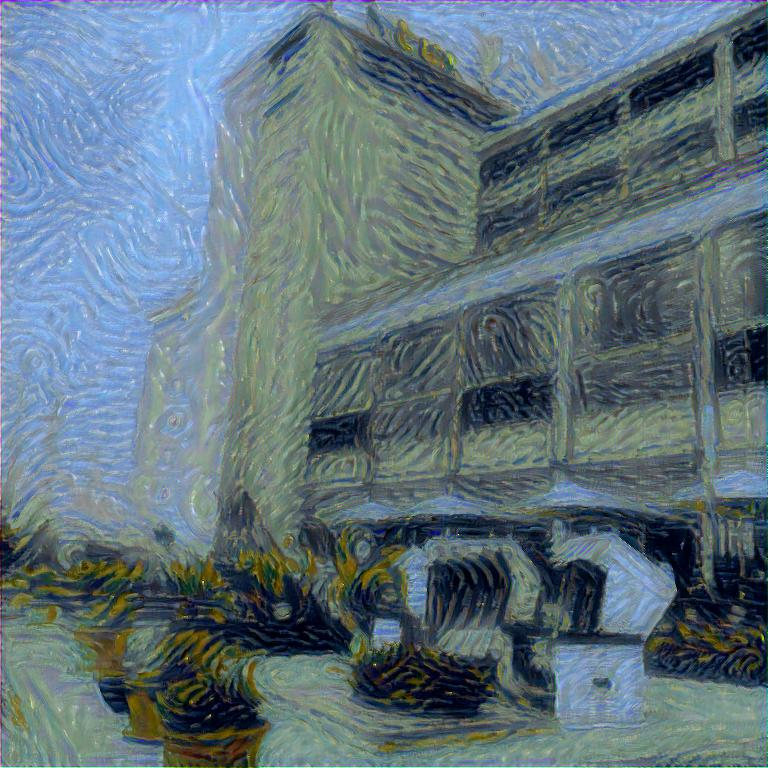
\includegraphics[width=\textwidth]{resources/content/experiments/a__starry_night__768x768__style-weight_1e+09__tv-weight_0e+00.jpg}
    \end{subfigure}
    \caption{Starry Night mit $ \alpha = 1 $, $ \beta = 10^{5} - 10^{9} $, $ \gamma = 0 $}
\end{figure}

In der zweiten Abbildungen werden verschiedene die verschiedenen Total-Variation-Gewichtungen $ \gamma = 10^{-7} $, $ \gamma = 10^{-6} $, $ \gamma = 10^{-5} $, $ \gamma = 10^{-4} $ und $ \gamma = 10^{-3} $  für Starry Night getestet.

\begin{figure}[H]
    \centering
    \begin{subfigure}[h]{0.15\textwidth}
        \centering
        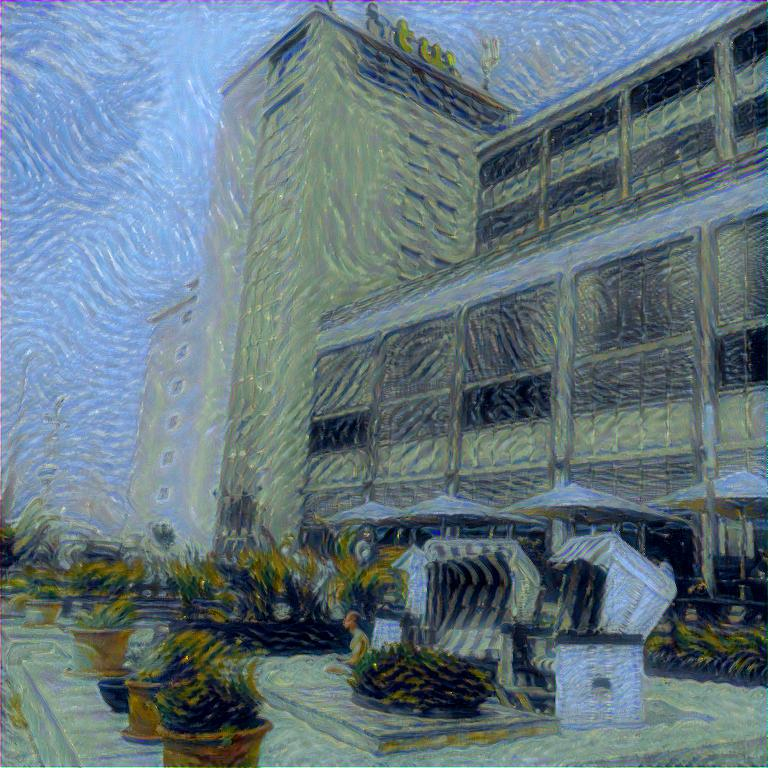
\includegraphics[width=\textwidth]{resources/content/experiments/b__starry_night__768x768__style-weight_1e+08__tv-weight_1e-07.jpg}
    \end{subfigure}
    \begin{subfigure}[h]{0.15\textwidth}
        \centering
        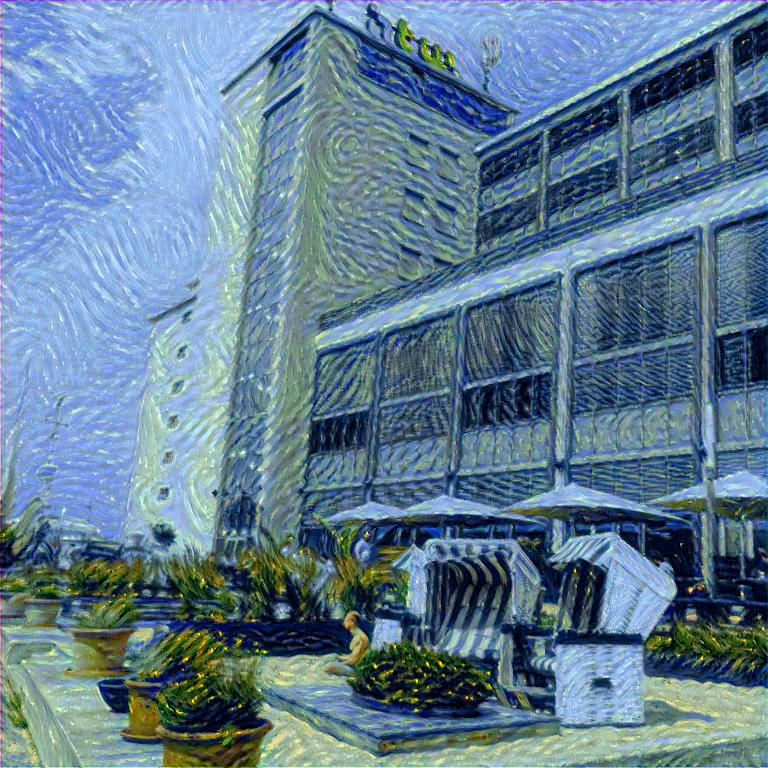
\includegraphics[width=\textwidth]{resources/content/experiments/b__starry_night__768x768__style-weight_1e+08__tv-weight_1e-06.jpg}
    \end{subfigure}
    \begin{subfigure}[h]{0.15\textwidth}
        \centering
        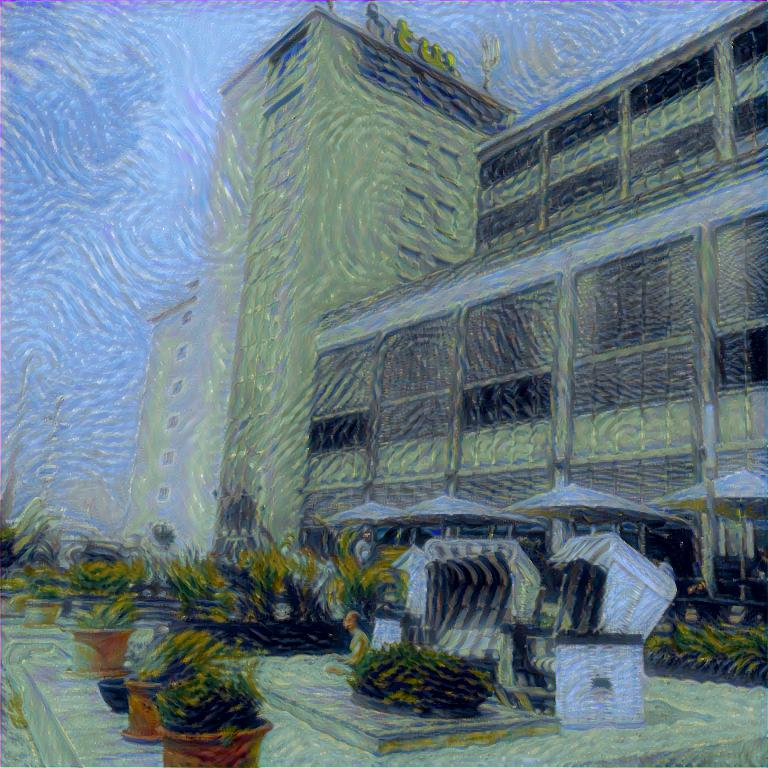
\includegraphics[width=\textwidth]{resources/content/experiments/b__starry_night__768x768__style-weight_1e+08__tv-weight_1e-05.jpg}
    \end{subfigure}
    \begin{subfigure}[h]{0.15\textwidth}
        \centering
        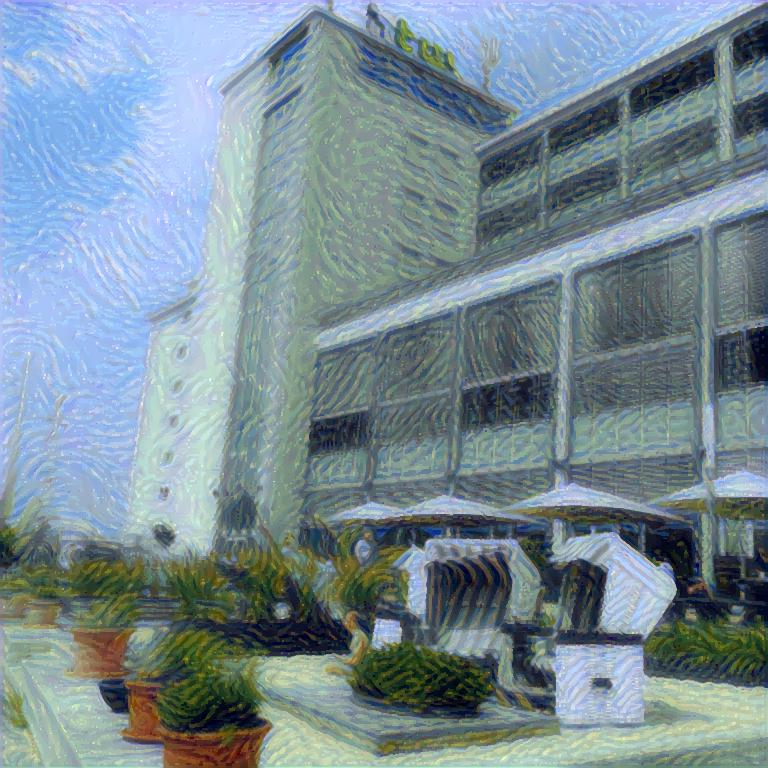
\includegraphics[width=\textwidth]{resources/content/experiments/b__starry_night__768x768__style-weight_1e+08__tv-weight_1e-04.jpg}
    \end{subfigure}
    \begin{subfigure}[h]{0.15\textwidth}
        \centering
        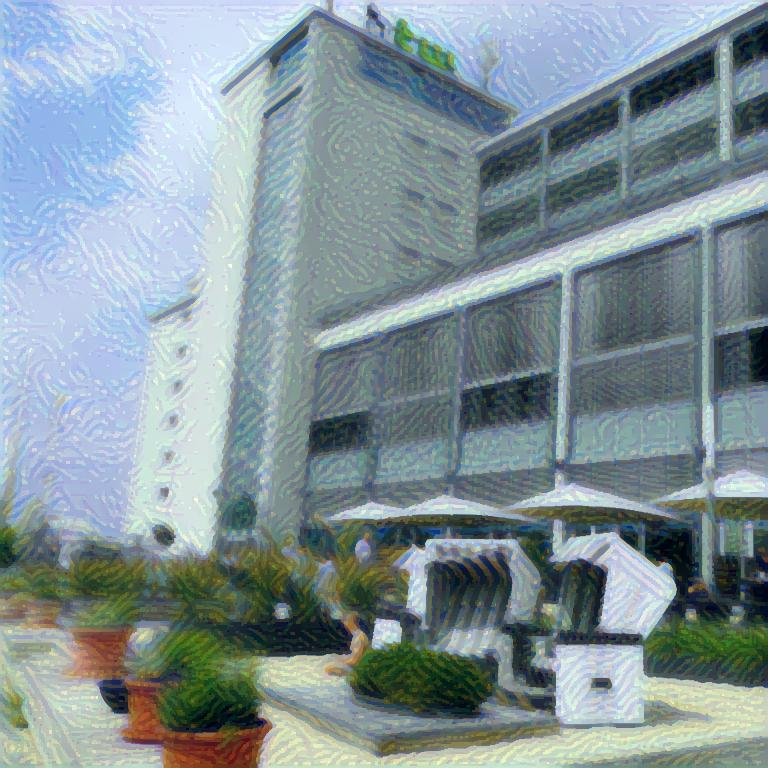
\includegraphics[width=\textwidth]{resources/content/experiments/b__starry_night__768x768__style-weight_1e+08__tv-weight_1e-03.jpg}
    \end{subfigure}
    \caption{Starry Night mit $ \alpha = 1 $, $ \beta = 10^{8} $, $ \gamma = 10^{-7} - 10^{-3} $}
\end{figure}

\pagebreak

\subsection{Experiment 2: The Scream}

\begin{figure}[H]
    \centering
    \begin{subfigure}[h]{0.20\textwidth}
        \centering
        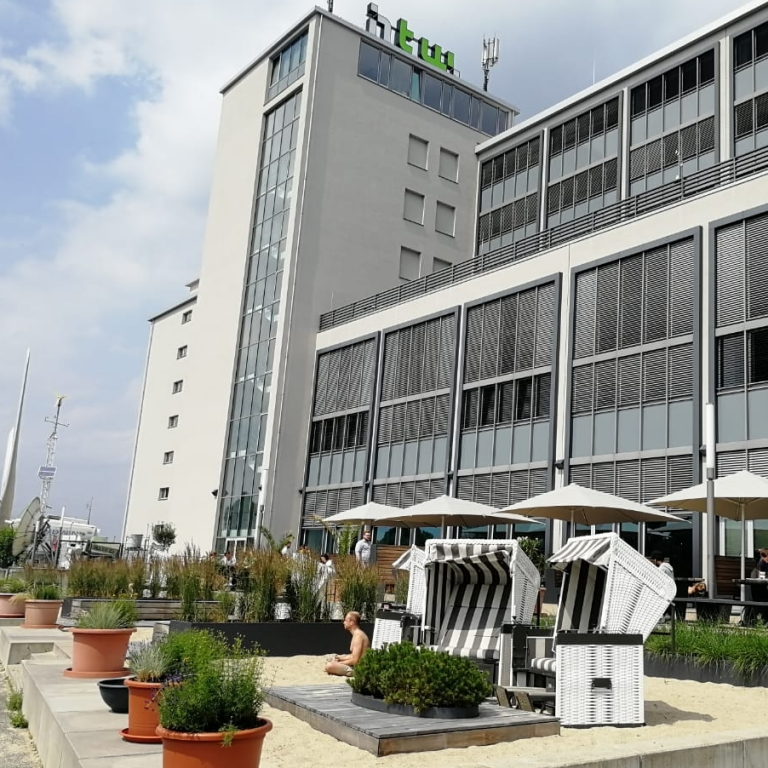
\includegraphics[width=\textwidth]{resources/content/content/htw-768x768.jpg}
    \end{subfigure}
    \begin{subfigure}[h]{0.20\textwidth}
        \centering
        \includegraphics[width=\textwidth]{resources/content/style/the_scream.jpg}
    \end{subfigure}
    \caption{HTW kombiniert mit The Scream}
\end{figure}


In der ersten Abbildungen werden verschiedene die verschiedenen  \\
Stilgewichtungen $ \beta = 10^{5} $, $ \beta = 10^{6} $, $ \beta = 10^{7} $, $ \beta = 10^{8} $ und $ \beta = 10^{9} $ für The Scream getestet.

\begin{figure}[H]
    \centering
    \begin{subfigure}[h]{0.15\textwidth}
        \centering
        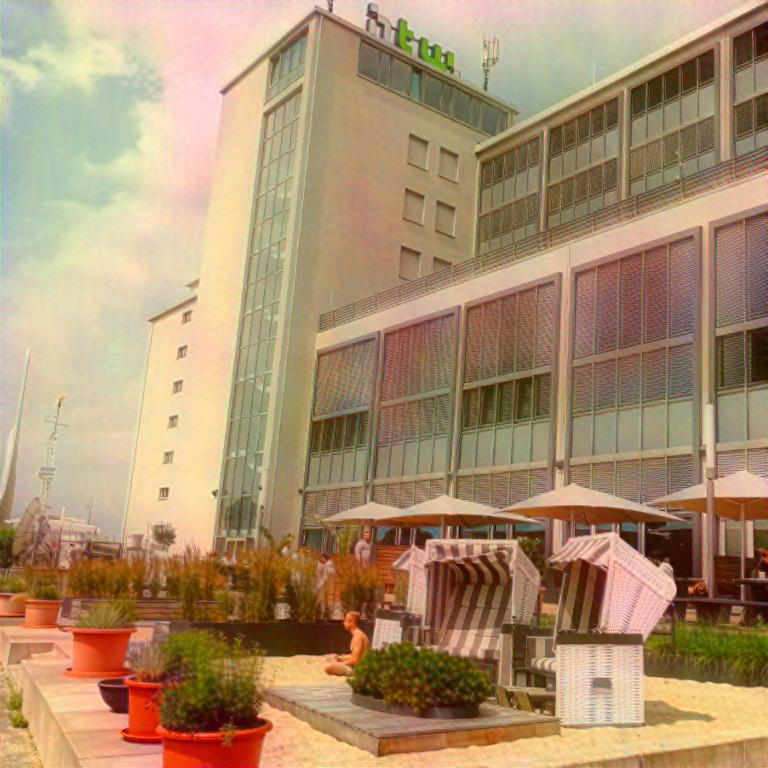
\includegraphics[width=\textwidth]{resources/content/experiments/a__the_scream__768x768__style-weight_1e+05__tv-weight_0e+00.jpg}
    \end{subfigure}
    \begin{subfigure}[h]{0.15\textwidth}
        \centering
        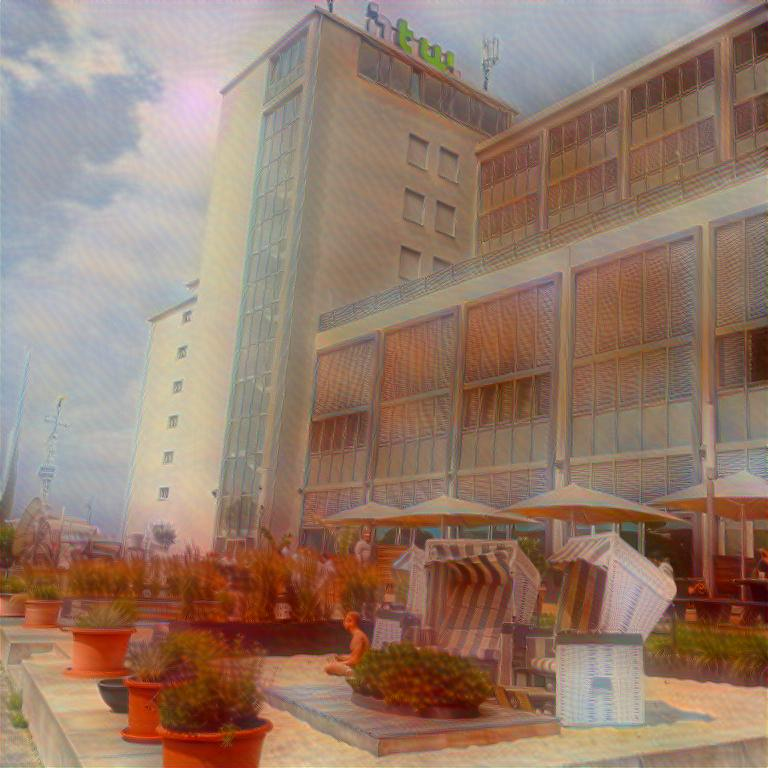
\includegraphics[width=\textwidth]{resources/content/experiments/a__the_scream__768x768__style-weight_1e+06__tv-weight_0e+00.jpg}
    \end{subfigure}
    \begin{subfigure}[h]{0.15\textwidth}
        \centering
        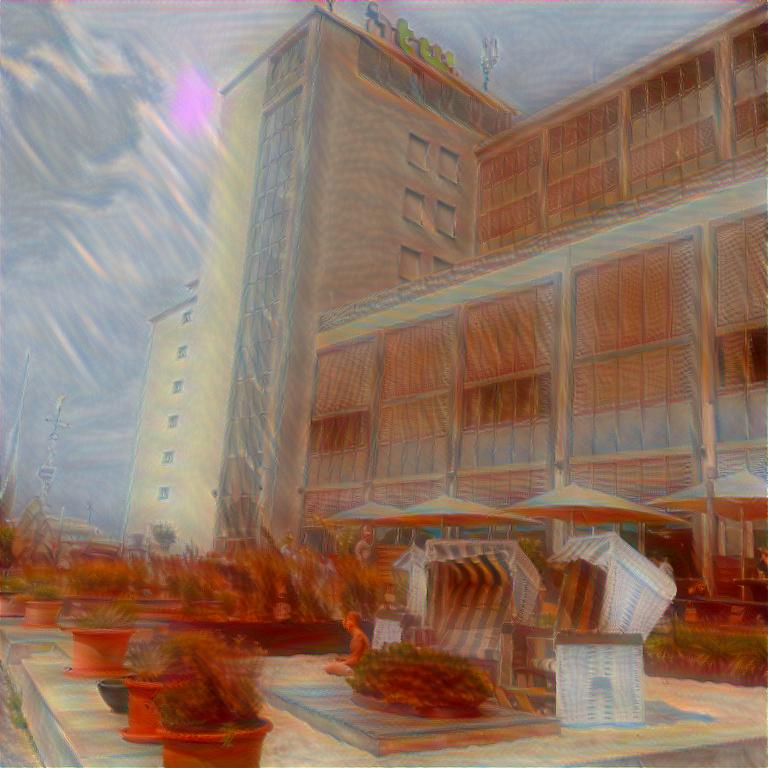
\includegraphics[width=\textwidth]{resources/content/experiments/a__the_scream__768x768__style-weight_1e+07__tv-weight_0e+00.jpg}
    \end{subfigure}
    \begin{subfigure}[h]{0.15\textwidth}
        \centering
        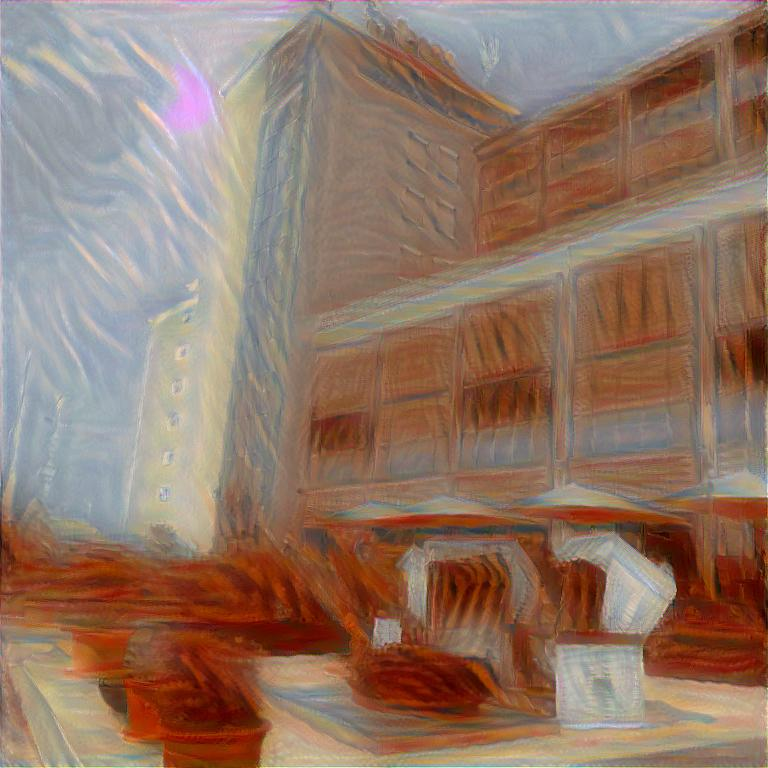
\includegraphics[width=\textwidth]{resources/content/experiments/a__the_scream__768x768__style-weight_1e+08__tv-weight_0e+00.jpg}
    \end{subfigure}
    \begin{subfigure}[h]{0.15\textwidth}
        \centering
        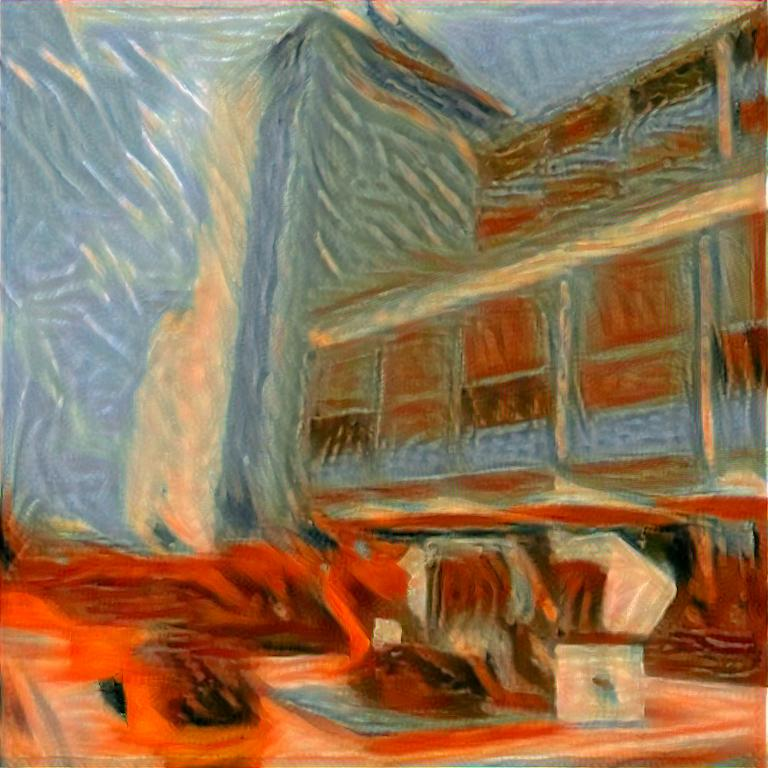
\includegraphics[width=\textwidth]{resources/content/experiments/a__the_scream__768x768__style-weight_1e+09__tv-weight_0e+00.jpg}
    \end{subfigure}
    \caption{The Scream mit $ \alpha = 1 $, $ \beta = 10^{5} - 10^{9} $, $ \gamma = 0 $}
\end{figure}

In der zweiten Abbildungen werden verschiedene die verschiedenen Total-Variation-Gewichtungen $ \gamma = 10^{-7} $, $ \gamma = 10^{-6} $, $ \gamma = 10^{-5} $, $ \gamma = 10^{-4} $ und $ \gamma = 10^{-3} $ für The Scream getestet.

\begin{figure}[H]
    \centering
    \begin{subfigure}[h]{0.15\textwidth}
        \centering
        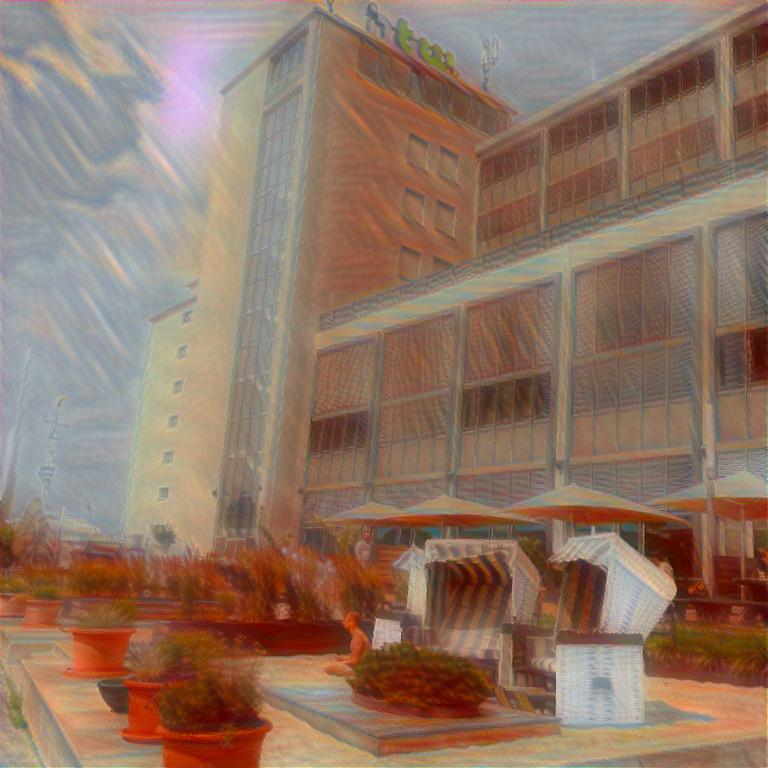
\includegraphics[width=\textwidth]{resources/content/experiments/b__the_scream__768x768__style-weight_1e+07__tv-weight_1e-07.jpg}
    \end{subfigure}
    \begin{subfigure}[h]{0.15\textwidth}
        \centering
        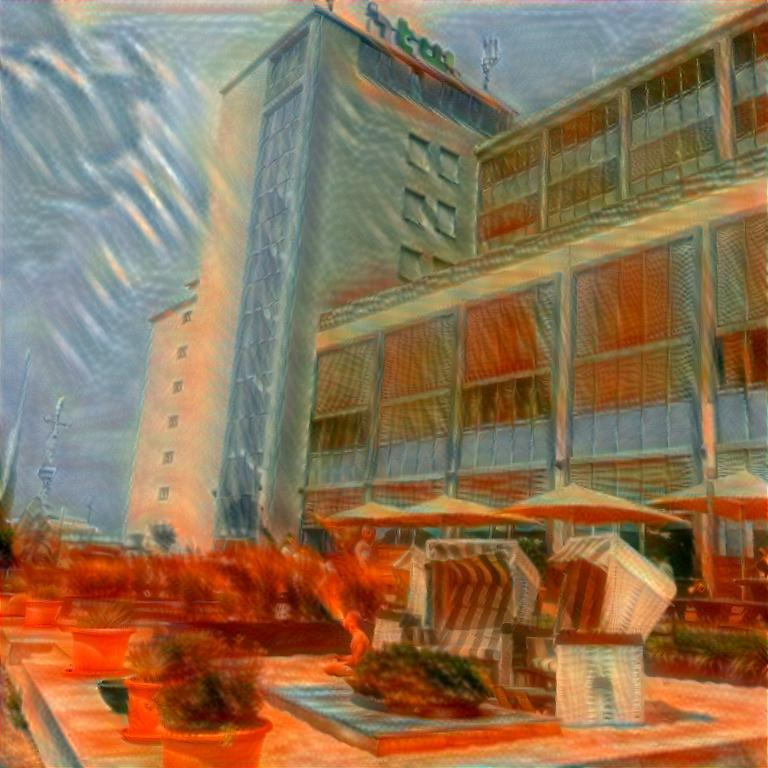
\includegraphics[width=\textwidth]{resources/content/experiments/b__the_scream__768x768__style-weight_1e+07__tv-weight_1e-06.jpg}
    \end{subfigure}
    \begin{subfigure}[h]{0.15\textwidth}
        \centering
        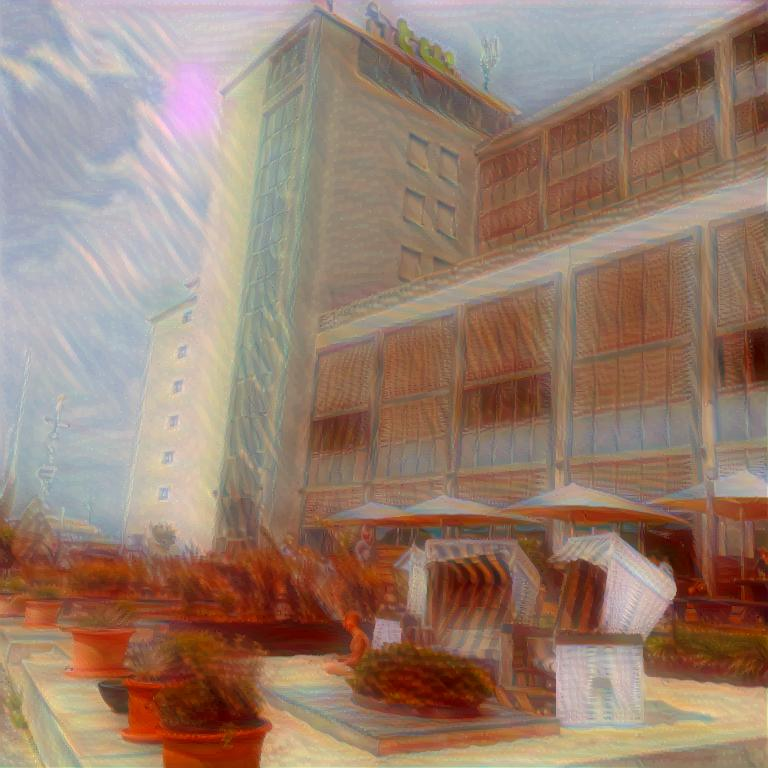
\includegraphics[width=\textwidth]{resources/content/experiments/b__the_scream__768x768__style-weight_1e+07__tv-weight_1e-05.jpg}
    \end{subfigure}
    \begin{subfigure}[h]{0.15\textwidth}
        \centering
        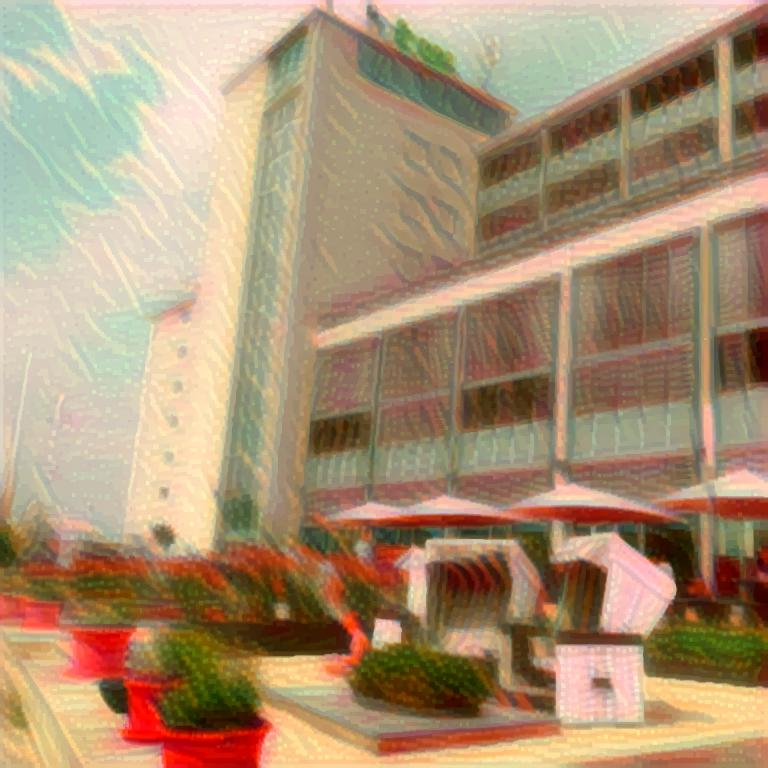
\includegraphics[width=\textwidth]{resources/content/experiments/b__the_scream__768x768__style-weight_1e+07__tv-weight_1e-04.jpg}
    \end{subfigure}
    \begin{subfigure}[h]{0.15\textwidth}
        \centering
        
\includegraphics[width=\textwidth]{resources/content/experiments/b__the_scream__768x768__style-weight_1e+07__tv-weight_1e-03.jpg}
    \end{subfigure}
    \caption{The Scream mit $ \alpha = 1 $, $ \beta = 10^{7} $, $ \gamma = 10^{-7} - 10^{-3} $}
\end{figure}

\pagebreak

\section{Auswirkungen der Netzwerkarchitekturen}

Im nächsten Experiment werden drei unterschiedlichen Bildgrößen auf unterschiedlichen Geräten auf Durchführbarkeit getestet.
Gemessen wird die Berechnungsgeschwindigkeit beim Forward-Pass durch das Netzwerk. 

Ein bereits erster Indikator für die Performanz eines Neurolen Netzwerks ist die Anzahl der lernbaren Parameter, die bei der Trainingsphase optimiert werden. Trainiert wurden neun unterschiedliche Netzwerke auf dem Kunstwerk \textit{Starry Night} mit Unterschiedlichen Kombinationen für $ m $ und $ s $

\begin{table}[H]
    \centering
    \begin{tabular}{ |c|c|c|c| }
        \hline
        \textbf{Name} & \textbf{Bottleneck Size $ s $} & \textbf{Multiplkator $ m $} & \textbf{Anzahl lernbarer Parameter} \\ \hline
        Netzwerk 1 & 5 & 32 & 2.006.931 \\ \hline
        Netzwerk 2 & 5 & 16 & 506.835 \\ \hline
        Netzwerk 3 & 5 & 8  & 129.267 \\ \hline

        Netzwerk 4 & 4 & 32 & 1.711.250 \\ \hline
        Netzwerk 5 & 4 & 16 & 432.722 \\ \hline
        Netzwerk 6 & 4 & 8  & 110.642 \\ \hline

        Netzwerk 7 & 3 & 32 & 1.415.569 \\ \hline
        Netzwerk 8 & 3 & 16 & 358.609 \\ \hline
        Netzwerk 9 & 3 & 8  & 92.017 \\ \hline
    \end{tabular}
    \caption{Unterschiedliche Netzwerkgrößen und ihre Parameter}
    \label{tab:networks}
\end{table}

Es macht dabei einen Unterschied ob die die Berechnung des Netzwerks auf dem CPU oder dem GPU eines Geräts durchgeführt wird. Neuronale Netzwerke können auf einer GPU besonders schneller als auf einem CPU berechnet werden. Das liegt daran eine GPU besonders auf die Berechnung von Matrix-Operationen (wie Sie auch bei Grafischen Anwendungen verwendet werden) spezialisiert ist.

Die Daten die werden beim einsatzt des GPUs in den Grafikspeicher geladen. Bei der Berechnung über den CPU wird der Arbeitsspeicher (RAM) des Geräts verwendet. Der RAM kann über die Verwendung einer Auslagerungsdatei (SWAP-Datei) virtuell erweitert werden. Somit kann verhindert werden das es zu Fehlern wegen unzureichendem Arbeitsspeicher kommt.

\begin{table}[H]
    \centering
    \begin{tabular}{ |c|c|c|c|c| }
        \hline
        \textbf{Name} & \textbf{XPS 15 - CPU} & \textbf{XPS 15 - GPU} & \textbf{Auto - CPU} & \textbf{Auto - GPU}   \\ \hline
        Netzwerk 1 & 1 sec & 1 sec & 1 sec & 1 sec \\ \hline
        Netzwerk 2 & 1 sec & 1 sec & 1 sec & 1 sec \\ \hline
        Netzwerk 3 & 1 sec & 1 sec & 1 sec & 1 sec \\ \hline
	
        Netzwerk 4 & 1 sec & 1 sec & 1 sec & 1 sec \\ \hline
        Netzwerk 5 & 1 sec & 1 sec & 1 sec & 1 sec \\ \hline
        Netzwerk 6 & 1 sec & 1 sec & 1 sec & 1 sec \\ \hline

        Netzwerk 7 & 1 sec & 1 sec & 1 sec & 1 sec \\ \hline
        Netzwerk 8 & 1 sec & 1 sec & 1 sec & 1 sec \\ \hline
        Netzwerk 9 & 1 sec & 1 sec & 1 sec & 1 sec \\ \hline
    \end{tabular}
    \caption{Berechnungsgeschwindigkeit für Bilder der Größe 1024 * 768 Pixel}
    \label{tab:1024x768}
\end{table}


\begin{table}[H]
    \centering
    \begin{tabular}{ |c|c|c|c|c| }
        \hline
        \textbf{Name} & \textbf{XPS 15 - CPU} & \textbf{XPS 15 - GPU} & \textbf{Auto - CPU} & \textbf{Auto - GPU}   \\ \hline
        Netzwerk 1 & 1 sec & 1 sec & 1 sec & 1 sec \\ \hline
        Netzwerk 2 & 1 sec & 1 sec & 1 sec & 1 sec \\ \hline
        Netzwerk 3 & 1 sec & 1 sec & 1 sec & 1 sec \\ \hline
	
        Netzwerk 4 & 1 sec & 1 sec & 1 sec & 1 sec \\ \hline
        Netzwerk 5 & 1 sec & 1 sec & 1 sec & 1 sec \\ \hline
        Netzwerk 6 & 1 sec & 1 sec & 1 sec & 1 sec \\ \hline

        Netzwerk 7 & 1 sec & 1 sec & 1 sec & 1 sec \\ \hline
        Netzwerk 8 & 1 sec & 1 sec & 1 sec & 1 sec \\ \hline
        Netzwerk 9 & 1 sec & 1 sec & 1 sec & 1 sec \\ \hline
    \end{tabular}
    \caption{Berechnungsgeschwindigkeit für Bilder der Größe 640 * 480 Pixel}
    \label{tab:640x480}
\end{table}


\begin{table}[H]
    \centering
    \begin{tabular}{ |c|c|c|c|c| }
        \hline
        \textbf{Name} & \textbf{XPS 15 - CPU} & \textbf{XPS 15 - GPU} & \textbf{Auto - CPU} & \textbf{Auto - GPU}   \\ \hline
        Netzwerk 1 & 1 sec & 1 sec & 1 sec & 1 sec \\ \hline
        Netzwerk 2 & 1 sec & 1 sec & 1 sec & 1 sec \\ \hline
        Netzwerk 3 & 1 sec & 1 sec & 1 sec & 1 sec \\ \hline
	
        Netzwerk 4 & 1 sec & 1 sec & 1 sec & 1 sec \\ \hline
        Netzwerk 5 & 1 sec & 1 sec & 1 sec & 1 sec \\ \hline
        Netzwerk 6 & 1 sec & 1 sec & 1 sec & 1 sec \\ \hline

        Netzwerk 7 & 1 sec & 1 sec & 1 sec & 1 sec \\ \hline
        Netzwerk 8 & 1 sec & 1 sec & 1 sec & 1 sec \\ \hline
        Netzwerk 9 & 1 sec & 1 sec & 1 sec & 1 sec \\ \hline
    \end{tabular}
    \caption{Berechnungsgeschwindigkeit für Bilder der Größe 320 * 240 Pixel}
    \label{tab:320x240}
\end{table}
